\documentclass[titlepage]{article}

\usepackage[utf8]{inputenc}
\usepackage[english]{babel} 
\usepackage{lineno, a4wide} % add line numbers
\linenumbers
\usepackage{setspace} % to use double spacing
\doublespacing

\usepackage{authblk} % author and affiliations
\usepackage{amssymb, amsmath} % for math formulas
\usepackage{bm}
\usepackage{amsfonts} % blackboard math symbols
\usepackage[round]{natbib} % citation format
\usepackage{hyperref} % creates links in the document
\usepackage{doi} % Create correct hyperlinks for DOI numbers
\usepackage{times} %Select Adobe Times Roman (or equivalent) as default font

\usepackage{graphicx} % handling figures
\usepackage{subfig} % handling figures
%\usepackage[nofiglist,figuresonly]{endfloat} % figures in the end
\usepackage[disable]{endfloat} % figures in the end
%\usepackage[nomarkers,figuresonly]{endfloat}
\usepackage{enumitem} % Control layout of itemize, enumerate, description
\usepackage{xcolor} % colored fonts

\usepackage[colorinlistoftodos]{todonotes} % to do comments

\usepackage{subfiles}
\usepackage{parskip}
\usepackage{multirow}
\usepackage[para,online,flushleft]{threeparttable}
\usepackage{rotating}
\usepackage{tikz}
\usepackage{tcolorbox}
\usepackage[none]{hyphenat} % no hyphenation in the end of lines
\usepackage[export]{adjustbox}[2011/08/13]

\title{
Estimating the cumulative impact and zone of influence of anthropogenic infrastructure on biodiversity  \\
{\normalsize Submitted manuscript}
}

% authors
\author[1,2,*]{Bernardo Brandão Niebuhr}
\author[1,*]{Bram Van Moorter} 
\author[3]{Audun Stien}
\author[4]{Torkild Tveraa}
\author[1]{Olav Strand}
\author[4]{Knut Langeland}
\author[5]{Per Sandström}
\author[6]{Moudud Alam}
\author[2]{Anna Skarin}
\author[1]{Manuela Panzacchi}

% affiliation
\affil[1]{Norwegian Institute for Nature Research (NINA), Trondheim, Norway}
\affil[2]{Swedish University of Agricultural Sciences (SLU), Uppsala, Sweden}
\affil[3]{University of Tromsø, Tromsø, Norway}
\affil[4]{Norwegian Institute for Nature Research (NINA), Tromsø, Norway}
\affil[5]{Swedish University of Agricultural Sciences (SLU), Umeå, Sweden}
\affil[6]{Dalarna University, Falun, Sweden}
\affil[*]{Joint first authorship}

\date{Running headline: Estimating cumulative impacts of infrastructure \\
Corresponding author: Bernardo Brandão Niebuhr \\Norwegian Institute for Nature Research, Postboks 5685 Torgarden, \\7485 Trondheim, Norway \\Contact: bernardo.brandao@nina.no, bernardo\_brandaum@yahoo.com.br \\ Word count: 7749 \\ \today}

\begin{document}

\maketitle

\begin{abstract}

\begin{enumerate}

    \item Infrastructure development often takes place in landscapes already affected by multiple anthropogenic disturbances. Typically, the impact of a given type of infrastructure is determined by computing the distance to the nearest feature only, ignoring potential cumulative impacts of multiple features on biodiversity. We propose an approach to assess whether and how multiple anthropogenic features lead to cumulative impacts.

    \item We derive a method to estimate the effect size and zone of influence (ZoI) of infrastructure, that allows us to quantify the impact based on the nearest feature only and the cumulative impact of multiple features of the same type. First, we use simulations and an empirical case to understand under which circumstances the estimated cumulative ZoI cannot be distinguished from the ZoI of the nearest feature only. Second, we illustrate the approach by quantifying and visualizing cumulative impacts of recreational facilities in Norway on habitat selection of wild reindeer, a species highly sensitive to anthropogenic disturbance. 

    \item Simulations show the ZoI of the nearest feature and the cumulative ZoI cannot be distinguished when the occurrence of features is rare and ZoI is small, and when features are clustered and ZoI is large. In our empirical analysis we found strong evidence of cumulative impacts of private cottages and tourist resorts on reindeer, with ZoI radii of 10 and 20 km, respectively. While the impact of a single private cottage was negligible, the cumulative impact of an aggregation of cottages could be larger than that of a tourist resort. Hence, measuring only the ZoI of the nearest private cottage would underestimate the impact of the widespread phenomena of cabin villages.

    \item The approach we developed allows to assess cumulative impacts of infrastructure on biodiversity, and can be broadly applied in impact assessment and land use planning. The ZoI metrics presented are computationally efficient and flexible and can be computed in R and GRASS GIS through the \verb|oneimpact| R package. Although our example focuses on animal space use, the approach can be applied
    in environmental impact studies from individuals to populations and communities, and counter the widespread trend of underestimating anthropogenic impacts.
\end{enumerate}

\textbf{Key-words:} Anthropocene, cumulative effects, distance-weighting, habitat fragmentation, habitat selection, kernel density, \textit{Rangifer tarandus}, scale of effect

\end{abstract}

\section{Introduction}

Land use change and infrastructure from industrial development are increasing at an accelerated pace across all regions of the world \citep{venter_sixteen_2016,ibisch_global_2016}, including all global biodiversity hotspots \citep{hu_overview_2021}, and are among the main causes of biodiversity declines \citep{benitez-lopez_impacts_2010,newbold_global_2015}. Most infrastructure development takes place in areas already affected by multiple sources of disturbance \citep{barber_roads_2014} and, thus, infrastructure of the same type are often clustered in the landscape. Understanding a species' response to spatially co-occurring infrastructure is crucial to adequately assess their total impact. Indeed, the impact of new anthropogenic features might add and spatially interact to that of preexisting ones, leading to a cumulative impact larger than that of 
single features in isolation \citep[Box 1; ][]{naugle_unifying_2011}.  
Adequately quantifying cumulative impacts is of crucial importance for ensuring ecological sustainability in land use planning, preventing habitat loss due to anthropogenic development, and informing robust mitigation or off-set measures \citep{gillingham_integration_2016, laurance_roads_2017}. Most environmental impact assessment studies focus on single infrastructure projects at small spatio-temporal scales \citep{johnson_regulating_2011}, and even broad-scale ecological studies typically consider only the impact of the nearest anthropogenic feature, ignoring cumulative impacts of multiple co-occurring features \citep[e.g.][]{torres_assessing_2016}. This relies on the assumption that only the infrastructure feature closest to the species' location matters, and that other co-occurring features have zero impact on the species. Although there have been increasing efforts to better define, review, and outline approaches for cumulative impact assessment \citep{naugle_unifying_2011,gillingham_integration_2016}, we still lack a comprehensive framework to quantify cumulative impacts and thus concretely help sustainable land use planning. We aim at contributing to fill this gap by proposing an approach to assess whether and how multiple anthropogenic features can lead to cumulative impacts, based on the assumptions that each feature has the same effect size, after controlling for spatial decay.

Anthropogenic infrastructure directly affects the area where they are built (e.g. through habitat loss or road kills), but might also affect species and ecological processes far beyond the infrastructure itself \citep[e.g. by causing avoidance responses and reducing the probability of animal occurrence in its proximity;][]{johnson_cumulative_2005,torres_assessing_2016,dorber_indicators_2022}. Therefore, two intrinsically related dimensions need to be assessed in impact studies: the effect size and the size of the affected area \citep[Box 1; ][]{naugle_unifying_2011}. The \textit{effect size} indicates how strongly a feature influences the focal species, and it is generally estimated through a combination of biological and environmental data via statistical modeling \citep[Box 1;][]{polfus_identifying_2011}. The \textit{zone of influence} (ZoI) 
corresponds to the area within which there are detectable impacts of the anthropogenic feature, and it is commonly expressed in terms of distances --- typically the radius delimiting the affected area \citep[Box 1;][]{polfus_identifying_2011,boulanger_estimating_2012}. 

The impact of co-occurring infrastructure of the same type -- our focus here -- can accumulate over space (and time), as a 
linear or non-linear function of the impact of each individual feature. Such cumulative impacts are commonly appraised by reclassifying infrastructure depending on scale -- e.g. many buildings together may be reclassified as an urban area and many wind turbines as a wind park \citep{torres_assessing_2016}.
When determining the ZoI, the concept of ecological threshold
has commonly been used \citep[see][and analytical procedures therein]{ficetola_ecological_2009}. Under this framework, the estimation of the ZoI is often carried out by modelling the response of a species as a function of distance to infrastructure using piece-wise regression or other non-linear regression models \citep[e.g. exponential decay or generalized additive models;][]{skarin_out_2018, ficetola_ecological_2009}, and typically only the distance to the nearest infrastructure is considered. This approach is generally limited to the assessment of ZoI thresholds for only one or a few types of infrastructure \citep[e.g.][]{boulanger_estimating_2012}, since its computation requires repeated fitting and becomes impractical in a broader context \citep{lee_estimating_2020}. 

Another approach used to estimate ZoI focuses on spatial and temporal \textit{scales of effect} in the evaluation of species-habitat relationships -- called multi-scale approaches \citep[e.g.][]{zeller_multi-level_2017}. In this context, the number of features is averaged for multiple spatial extents surrounding the focal study sites \citep{jackson_are_2015} or considering different grains \citep{laforge_process-focussed_2015}, or weighted using neighborhood analysis over several different extents or radii (generally termed \textit{scales}), creating a series of infrastructure density maps \citep{mcgarigal_multi-scale_2016}. Spatial extents and grains are typically linked to the spatial and temporal dimensions of the infrastructure considered, as well as to the expected scale of the biological response to such infrastructure. Each of these maps are tested against the response variables to assess the extent at which the relationship is the strongest, most commonly through measures of model performance and explanatory power such as R\textsuperscript{2}, AIC, or BIC, or by evaluating the variation in fitted model coefficients \citep{jackson_are_2015, huais_multifit_2018}.
Multi-scale analyses brought important advances to landscape and environmental impact studies \citep[e.g.][]{mcgarigal_multi-scale_2016}, even though in many cases the scale of effect was not properly evaluated \citep{jackson_are_2015}. However, these approaches are rarely put into the framework of cumulative impact assessment \citep[but see][]{polfus_identifying_2011}.

We propose an approach to detect the occurrence of cumulative impacts and quantify them assuming additive effects of multiple features, empirical estimates of effects sizes, and a model selection approach to determine the ZoI, which defines the functional form of the decreasing impact with distance. The model approach allows estimation of both the impact based on the nearest features only, and the cumulative impact of multiple features (Box 1, Fig. \ref{fig:zoi_conceptual}). First, we perform simulations to understand under which conditions these two estimates of impact represent similar spatial gradients.
Second, we illustrate our approach by assessing the cumulative impacts of recreational housing facilities (private cottages and tourist resorts) in Norway on habitat selection of the tundra's flagship species, reindeer (\textit{Rangifer tarandus tarandus}). We provide tools to allow easy implementation of the approach in R \citep{r_core_team_r_2020} or GRASS GIS \citep{grass_development_team_geographic_2017} through the \verb|oneimpact| R package. This approach allows us to: (i) quantify the cumulative impact of multiple features of an infrastructure type; (ii) evaluate whether there is evidence for cumulative impacts, or whether the impact of the nearest feature sufficiently captures the species' response to infrastructure; and (iii) estimate the impact and ZoI of multiple types of infrastructure. 

\begin{tcolorbox}[width=1.3\textwidth,center,colback=yellow!5,colframe=yellow!75!black,title={Box 1 -- Definitions}]

\begin{description}

    \item[Impact] We use the term to represent the consequences of industrial landscape changes on a focal biological response variable, such as measures of biodiversity or ecological processes. Thus, impacts represent the functional responses of species and processes to human activity \citep{naugle_unifying_2011}. We analytically decompose the impact $I$ into its \textbf{effect size $\beta$} and its spatial component, the \textbf{zone of influence (ZoI) $\phi$}, so that $I = \beta \cdot \phi$. A given infrastructure feature (e.g. tourist cabin) might affect a certain process (e.g. an species occurrence) strongly or weakly ($\beta$), and this impact might decrease fast with distance or extend over several kilometers (ZoI, $\phi$).
    
    \item[Cumulative impacts] can result from the interaction between multiple features of an infrastructure -- our focus here --, from the impact of different types of infrastructure (e.g. houses, turbines, roads, dams) or from top-down or bottom-up ecological cascades. Cumulative impacts of multiple features depend on the number of features in an area, their spatial distribution, and co-occurrence with other infrastructure types, and might differ for distinct species, values, or processes -- possibly leading to stronger negative impacts for some or even to benefits for others, if compared to the impact of single, isolated infrastructure.
    
    \item[Effect sizes] express how strongly a given biological response is affected by a type of disturbance at the point in space where the disturbance is located. Here, the effect size is given by the estimated model coefficients $\beta$ (eq. \ref{eqn:HSF}).
    
    \item[Zone of Influence] The \textbf{ZoI} represents the function $\phi$ defining how the effect size of an infrastructure feature changes with the distance, i.e. it represents how the impact spreads throughout space. The ZoI might be any function $\phi(d, r)$ that assumes value 1 at the origin and decreases towards zero as the distance $d$ from infrastructure increases. The ZoI is defined by its \textbf{shape} and \textbf{radius \textit{r}}. The ZoI \textbf{shape} determines how $\phi$ decreases with distance, or whether it is constant up to a threshold distance $r$ (see Fig. \ref{fig:zoi_conceptual}A and Appendix A for examples). The ZoI \textbf{radius $r$} is the maximum distance from infrastructure where it affects a given biological response. For some shapes (e.g. threshold, linear decay) $r$ is the distance at which $\phi$ reaches zero (Fig. \ref{fig:zoi_conceptual}A). For non-vanishing functions (e.g. Gaussian decay), a cutoff must be set to define $r$ -- e.g. the minimal distance where $\phi$ is below 0.05. 
    While in landscape ecology the ZoI radius is often called the \textit{scale of effect} \citep[e.g.][]{jackson_are_2015}, we use the term ZoI to avoid confusion from different definitions of \textit{scale}.
    
    \item[ZoI metrics] When multiple features of an infrastructure are present, we can compute two ZoI metrics: the ZoI of the nearest feature only ($\phi_{nearest}$, eq. \ref{eqn:HSFnearest}) and the cumulative ZoI of multiple features ($\phi_{cumulative}$, eq. \ref{eqn:HSFcuminf}), which is the sum of each features ZoI (Fig. \ref{fig:zoi_conceptual}B).
    
\end{description}
\end{tcolorbox}

\section{Defining cumulative impact and ZoI for multiple features}

We first derive a measure for the impact of multiple features of an infrastructure type, e.g.\ roads or houses, on biological response variables. To illustrate this, we use habitat selection analysis, where the aim is to discriminate which environmental conditions are selected or avoided by animals. This is based on ecological data such as species occurrence or movement data and use-availability designs \citep{fieberg_how_2021}. The main element in habitat selection approaches is the habitat selection function (HSF) $w(\textbf{X},\textbf{Z})$, a function proportional to the probability of selection of a given space resource unit, estimated from the frequency of used and available resource units \citep{thurfjell_applications_2014}. The HSF $w(\textbf{X},\textbf{E})$ is function of a matrix of spatial predictor variables describing infrastructure, $\textbf{X}$, for which we want to estimate the impact and ZoI, and a matrix of other environmental variables, $\textbf{E}$ (e.g. temperature, vegetation type, altitude, or topography). In its parametric form, the HSF might be represented by

\begin{equation}
\centering
\label{eqn:HSFgeneral}
    w(\textbf{X},\textbf{E}) = \exp (\textbf{X} \bm{\beta} + \textbf{E} \bm{\alpha})
\end{equation}

where \bm{$\beta$} and \bm{$\alpha$} are vector of coefficients for $\textbf{X}$ and $\textbf{E}$. The first term can be written in vector form

\begin{equation}
\centering
\label{eqn:HSF}
    w(\textbf{X}) = \exp \left( \beta_0 + \overbrace{\beta_1 X_1}^\text{A) Infrastructure type 1} + \overbrace{\beta_2 X_2}^\text{B) Infrastructure type 2} + \underbrace{\beta_{12} X_1 X_2}_\text{D) Interaction infrastructure types 1 and 2} + ... + \overbrace{\beta_k X_k}^\text{C) Infrastructure type k} \right)
\end{equation}

where we define each term $I_k = \beta_k X_k$ as the \textit{impact} of a given infrastructure of type $k$, where the impact is decomposed into its effect size $\beta_k$ and a spatial component $X_k$. In terms of ecological interpretation, $\exp(\beta_k)$ might be understood as the relative selection strength \citep{avgar_relative_2017}, and $\exp(I_k)$ as how this relative selection strength varies in space, for infrastructure type $k$ \citep{fieberg_how_2021}.

In this formulation, \textit{the cumulative impact of different types of infrastructure} is given by the additive impacts of the $k$ infrastructure types (e.g. terms A, B, and C in equation \ref{eqn:HSF}) and possibly by interaction terms between variables (such as term D in equation \ref{eqn:HSF}, with an interaction coefficient $\beta_{12}$), that allows for non-linear, joint effects caused by the co-occurrence of different types of infrastructure. 

In our definition of impact, $\beta$ and $X$ are independent and \textit{the cumulative impact of multiple features the same infrastructure type} is determined by the spatial component of the impact, $X$. We start by verbally defining the ZoI as a function $\phi$, a curve that represents how the infrastructure impact changes with distance (Box 1). The ZoI of each infrastructure feature might follow different shapes -- it can be either constant (threshold ZoI) or decrease with distance from infrastructure (e.g. linear and Gaussian ZoI, Fig. \ref{fig:zoi_conceptual}A). More broadly, $\phi = f(d, r)$ is any decay function that has a maximum value 1 where the infrastructure is located and decreases towards zero as the Euclidean distance $d$ increases, and possibly vanishes at a given point, the ZoI radius $r$ (Box 1, Appendix A). Determining the ZoI shape and radius is an empirical problem \citep{miguet_how_2017}. The simplest assumption, widely used in the literature, is that all the area within the ZoI is affected equally \citep[a buffer zone around features; e.g][]{quinonezpinon_design_2007}, even though it might be more reasonable to consider that $\phi$ is higher close to infrastructure \citep[][]{skarin_out_2018, zeller_multi-level_2017}. 

When there are multiple features of an infrastructure we can define two ZoI metrics: the ZoI based on the nearest feature alone, $\phi_{nearest}$, and the cumulative ZoI of multiple features, $\phi_{cumulative}$ (Box 1, Fig. \ref{fig:zoi_conceptual}B). For $\phi_{nearest}$, the ZoI is assumed to be similar when approaching an isolated house and a small village, while for $\phi_{cumulative}$ the ZoI of nearby houses adds up and will be greater than that of a single, isolated house (Fig. \ref{fig:zoi_conceptual}B).

\begin{figure}[!htbp]
\centering
\includegraphics[width=0.9\textwidth]{figures/ZoI_conceptual_new.png}
\caption{\label{fig:zoi_conceptual} Illustration of the ZoI of infrastructure features in one dimensional space, using houses as example. (A) Examples of ZoI functions $\phi$ with different shapes of decay with distance from feature, $d$. A house has only an influence within its ZoI radius (here $r = 3 \text{ km}$). For the threshold function, the influence remains constant within the ZoI and drops to zero beyond it, whereas for both the linear and Gaussian functions it declines monotonically for $d \leq r$. 
(B) Representation of the ZoI of multiple houses by considering only the nearest feature ($\phi_{nearest}$, upper row) or the cumulative ZoI of multiple features ($\phi_{cumulative}$, bottom row), for different shapes. If only the nearest house is considered, $\phi_{nearest}$ does not exceed one; when all houses act cumulatively, $\phi_{cumulative}$ can be much higher than one.}
\end{figure}

To translate those representations into a mathematical form, now we decompose each of the impact terms (i.e. A, B, C, ...), in equation \ref{eqn:HSF}. Suppose that in the landscape there are $n_k$ features of the same type of infrastructure $k$, and let the ZoI of feature $i$ of an infrastructure $k$ follow $\phi_{i_k} = f(d_{i_k}; r_k)$, where $d_{i_k}$ is the distance to feature ($i_k$) and $r_k$ is its ZoI radius. We can sum the effect of each feature on animal habitat selection, so that the impact terms in equation \ref{eqn:HSF} become:

\begin{equation}
\label{eqn:HSFterm}
    I_k = \beta_k X_k = \sum_{i=1}^{n_k} \beta_{i_k} \phi_{i_k}
\end{equation}

Typically, only the nearest feature is considered, resulting on the implicit assumption that $\beta_i = 0$ for all but the nearest feature. Thus, eq. \ref{eqn:HSFterm} turns into:

\begin{equation}
\label{eqn:HSFnearest}
\begin{split}
    I_k & = \beta_{1_k} \phi_{1_k} \\
        & = \beta_{1_k} \phi_{nearest_k}
\end{split}                
\end{equation}

where $\phi_{nearest_k}$ is the ZoI of the nearest feature ($i = 1$) of the infrastructure type $k$ (see Fig. \ref{fig:zoi_conceptual}B). However, possibly a more reasonable assumption would be that $\beta_{i_k} = \beta_{{(i+1)}_k} = ... = \beta_k$, i.e. that all features of a given type present the same ZoI and all $\beta$'s are identical. Thus, eq. \ref{eqn:HSFterm} is reduced to:

\begin{equation}
\label{eqn:HSFcuminf}
\begin{split}
    I_k & = \beta_k \sum_{i=1}^{n_k} \phi_{i_k} \\
        & = \beta_k \phi_{cumulative_k}
\end{split}
\end{equation}

where $\phi_{cumulative_k} = \sum_{i} \phi_{i_k}$ is the cumulative ZoI metric and is proportional to 
the ``density" of features in space \citep[e.g.][]{panzacchi_searching_2015}. The cumulative ZoI metric is easily calculated using geographical information systems, e.g. through neighborhood analysis, and can be rescaled to meaningful scales, such as the number of houses (or length of roads) per km\textsuperscript{2}. For the derivation of similar equations for variables represented as lines and areas, see Appendix A.

\section{Estimating the cumulative impact of multiple features}

In the cumulative impact assessment proposed here, the calculation of the ZoI ($\phi$) is done before statistical analysis. In this formulation, $\phi$ defined based on different shapes and radii are considered as different covariates (Fig. \ref{fig:workflow}). Therefore, the evaluation of how the impact of multiple infrastructure features accumulate and the identification of the ZoI shape and size are recasted as a model selection rather than a parameterization problem \citep[such as in][]{lee_estimating_2020}.

\begin{figure}[h]
\centering
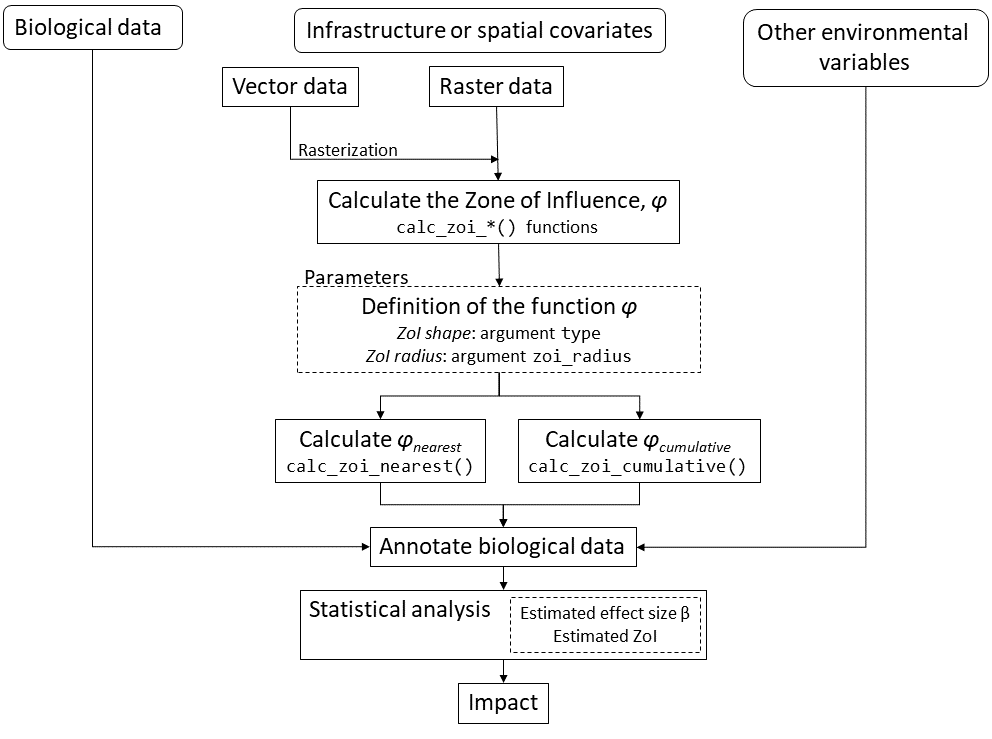
\includegraphics[width=1.3\textwidth,center]{figures/figure_workflow.png}
\caption{\label{fig:workflow} Workflow for calculating infrastructure ZoI $\phi$ and estimating the cumulative impact and ZoI radius of multiple infrastructure. Infrastructure raster data are input to the \texttt{calc\_zoi} functions, which allow the calculation 
of $\phi_{nearest}$ and $\phi_{cumulative}$ based on arguments for the ZoI shape and radius. The output influence rasters and other environmental data are then annotated to biological data, and for each infrastructure type each ZoI measure defined by a shape, radius, and metric is considered as a different covariate. The annotated data is then analyzed to estimate $\beta$ and $r$ for each infrastructure type and calculate the impact $I$.}
\end{figure}

To ease the use of the approach, we developed the \verb|oneimpact| R package. Based on raster maps with the location of infrastructure or other spatial variables, it allows the calculation of $\phi_{nearest}$ and $\phi_{cumulative}$ through the \verb|calc_zoi| functions (Fig. \ref{fig:workflow}, Appendix D). The output influence raster maps are then used with other environmental data to annotate biological data (e.g. GPS locations or sampling points), and the estimation of the effect sizes $\beta$ and evaluation of the cumulative effects for different types of infrastructure is made through statistical fitting of eq. \ref{eqn:HSFgeneral} (Fig. \ref{fig:workflow}). Statistical analyses can make use of model selection \citep{burnham_model_2002,huais_multifit_2018}, penalized regression \citep{lee_estimating_2020}, or machine learning approaches, for example \citep{james_introduction_2021}. Such statistical modeling procedures are beyond our scope, and we provide an example using model selection through AIC. See Appendix D for an introduction on how to use the \verb|oneimpact| package in R.

\section{When do $\phi_{nearest}$ and $\phi_{cumulative}$ represent similar spatial variation?}

To interpret the two ZoI metrics -- $\phi_{nearest}$ and $\phi_{cumulative}$ -- in ecological contexts, is it important to investigate in which conditions they are correlated and represent similar or different gradients of spatial variation. Similarities between the two variables depend on the spatial distribution of features as well as their ZoI, and might affect our ability to distinguish among their impacts. To illustrate when they converge, we simulated $30 \times 30$ km\textsuperscript{2} landscapes with 100m resolution and a constant number of point features ($n = 100$) distributed following different spatial patterns, in a gradient of clustering, from regular and random to clustered (Fig. \ref{fig:simulated_landscapes}; Appendix B). For each landscape we calculated $\phi_{nearest}$ and $\phi_{cumulative}$ assuming a range of values for ZoI radius (from 0.06\% to 40\% of the landscape extent), using a linear decay ZoI (Fig. \ref{fig:zoi_conceptual}). We then compared the resulting spatial patterns of $\phi_{nearest}$ and $\phi_{cumulative}$ through Pearson correlation of the values of the two metrics at the same coordinates. 

\begin{figure}[h]
\centering
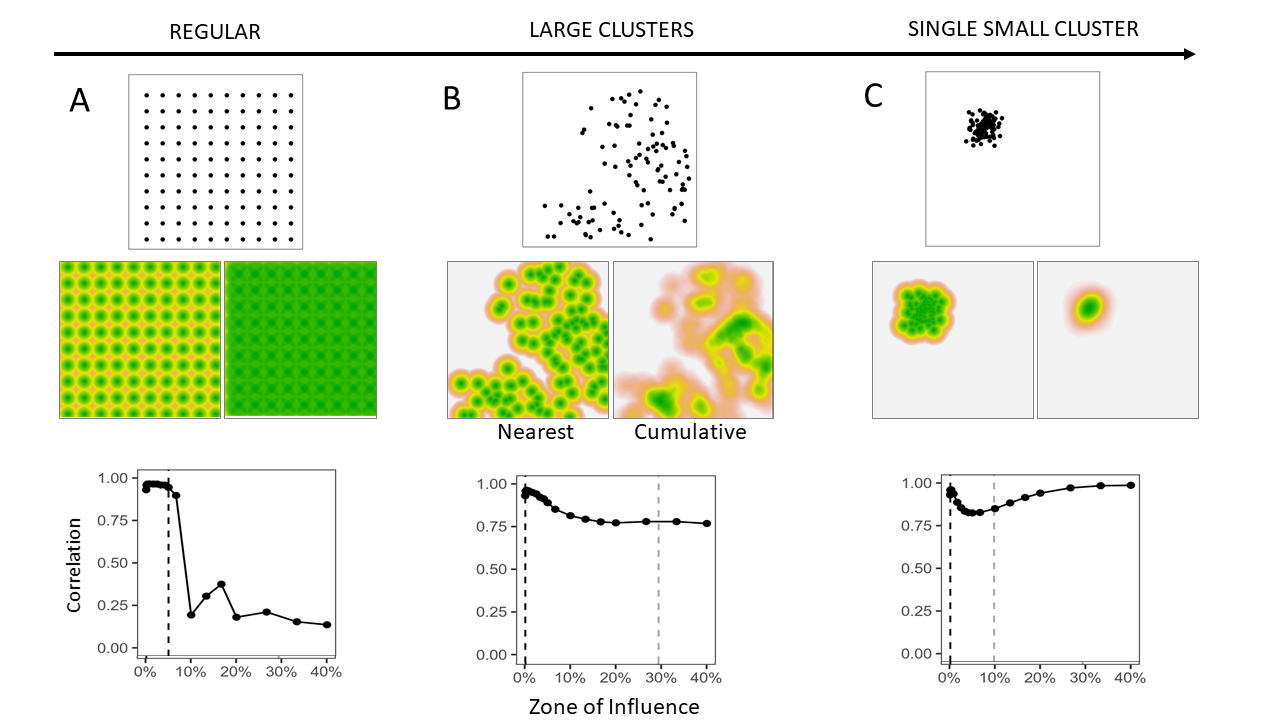
\includegraphics[width=1.3\textwidth,center]{figures/simulated_landscapes.png}
\caption{\label{fig:simulated_landscapes} Representation of the ZoI of nearest feature ($\phi_{nearest}$) and the cumulative ZoI ($\phi_{cumulative}$) in landscapes with point infrastructure spatially distributed in a gradient of clustering, from (A) a regular distribution to (B) a set of clusters to (C) only one cluster. 
The central panel shows a visual comparison between $\phi_{nearest}$ (left) and $\phi_{cumulative}$ (right) when the ZoI radius $r = 10\%$ of the landscape extent. The lower panel shows the correlation between $\phi_{nearest}$ and $\phi_{cumulative}$ in each landscape, as ZoI radius $r$ increases. The dashed vertical lines show half the the minimum distance between features (black), beyond which the ZoI of multiple infrastructure overlap, and the size of the feature clusters (grey), beyond which the correlation stops decreasing.}
\end{figure}

When the minimum distance between features is greater than $2r$, $\phi_{nearest}$ and $\phi_{cumulative}$ are identical (Fig. \ref{fig:simulated_landscapes}, black dashed vertical line; $\text{correlation} = 1$). This is because the ZoI of each feature is too restricted to overlap. When the ZoI radius increases, the effect of nearby features accumulate and the correlation between $\phi_{nearest}$ and $\phi_{cumulative}$ decreases (Fig. \ref{fig:simulated_landscapes}A,B, Figs B5 and B8). In addition, as the features get more aggregated (up to a limit with a single small cluster, Fig. \ref{fig:simulated_landscapes}C), the correlation between $\phi_{nearest}$ and $\phi_{cumulative}$ goes through a point of inflection as the ZoI expands, beyond which it increases with $r$ (Fig. B5D-F). The point where the correlation stops decreasing is related to the size of the clusters (grey dashed vertical line in Figs. \ref{fig:simulated_landscapes}B,C). For ZoI radius values larger than the radius of the cluster, $\phi_{nearest}$ and $\phi_{cumulative}$ converge again 
and it might be hard to distinguish between the effect of each feature alone, regardless of the ZoI metric; at this point the effect of a collection of features transforms into that of a ``super-feature" (e.g. urban areas instead of houses, wind parks instead of wind turbines). 
%While a high correlation between $\phi_{nearest}$ and $\phi_{cumulative}$ imply that it will be be difficult to distinguish if the impacts of a given infrastructure type accumulate or not, whether a given biological response variable is affected by the nearest feature or cumulatively by multiple features remains a question to be explored empirically. 

\section{Empirical demonstration on reindeer habitat selection}

\subsection{Material and methods}

In our empirical demonstration we assessed the impacts of multiple infrastructure on the Hardangervidda reindeer population in Norway using habitat selection during summer (Fig. \ref{fig:prediction_maps}). Reindeer are sensitive to human activity, and the populations in Norway are the last remaining wild reindeer populations in Europe. In summer, the area is visited by tourists and mountain hikers. There are 14,154 private cottages, 26 large tourist cabins, and hundreds of kilometers of trails in the area, besides roads and small tourist cabins (Fig. C2). We used GPS-tracking data from 115 female reindeer collected in the period of 1 July - 15 August from 2001 to 2019 \citep[see][for further details]{panzacchi_searching_2015}. To assess reindeer habitat selection, we used an use-availability setup, where each used GPS location was compared against nine available random locations spread within the area occupied by the population (Fig. \ref{fig:prediction_maps}). All locations were annotated with environmental covariates.

To account for bio-climatic-geographical variation in environmental characteristics we used the four first components from a principal component (PC) analysis conducted for whole Norway \citep{bakkestuen_step-less_2008}. They correspond to gradients of (1) PC1 - continentality, (2) PC2 - altitude, (3) PC3 - terrain ruggedness, and (4) PC4 - solar radiation. We included a quadratic term for PC1 and PC2 to account for niche ``optima" \citep[\textit{sensu}][]{panzacchi_searching_2015}. We also used a satellite-based land cover map with 25 vegetation classes, which were reclassified into 12 classes (see Table C2). To keep model fitting relatively simple and avoid correlation between covariates, we estimated the cumulative impact for two anthropogenic variables: private cottages and large tourist cabins.

For the two infrastructure types we calculated both $\phi_{nearest}$ and $\phi_{cumulative}$ (Fig.~\ref{fig:zoi_conceptual}B) for ZoI radii irregularly distributed in the range [100m, 20,000m]. For each ZoI, we used four ZoI shapes: threshold, linear decay, Gaussian decay, and exponential decay (Appendix A). To estimate reindeer habitat selection, we fitted HSFs (eq. \ref{eqn:HSF}) using binomial generalized linear models \citep{fieberg_how_2021} with used and available locations as response and infrastructure, land cover, and bio-climatic variables as fixed effects. 

Model fitting consisted in two steps. We first fitted single-infrastructure models using a variable selection procedure \citep{burnham_model_2002} to find the most likely ZoI (shape, radius) for each infrastructure type. Single-infrastructure HSF were fitted using the \verb|multifit| function in R \citep{huais_multifit_2018} and compared using AIC. Second, using the most likely ZoI from single-infrastructure models, we fitted multi-infrastructure HSF to assess the combined impacts of multiple types of infrastructure, in an approach similar to \citet{laforge_process-focussed_2015}. 

To quantify the impacts of infrastructure, we applied eq. \ref{eqn:HSFterm} using the $\beta$ and $\phi$ estimated from the model with lowest AIC. We then estimated habitat suitability predicting the HSF (eq. \ref{eqn:HSF}) over the study area and rescaling the predicted values to the interval [0, 1]. For details on data, environmental covariates, modeling, and results, see Appendix C.

\subsection{Results}

Overall, both single- and multi-infrastructure models including $\phi_{cumulative}$ performed much better than models including $\phi_{nearest}$ (Table C2). This presents strong evidence that the impacts of private cottages and tourist cabins accumulate over reindeer habitat selection, making them avoid these infrastructure types. As a comparison, the most plausible model including $\phi_{nearest}$ was ranked 26\textsuperscript{th} in the model selection ($\Delta AIC = 921$), and the most likely model including the log-distance to the nearest feature was ranked 44\textsuperscript{th} ($\Delta AIC = 1197$, Table C2).

The most parsimonious model showed private cottages exerted a constant cumulative impact within a threshold ZoI of 10 km and large tourist cabins followed an exponentially decaying cumulative ZoI with 20 km radius (Fig. \ref{fig:impact_plot}; Table C2). Notice that, as parameterized here, for the tourist cabins an exponential decay with ZoI of 20 km means
that the impact of tourist cabins decreases to half of its maximum value
at 5 km from the infrastructure (Fig. \ref{fig:impact_plot}, Appendix A). 

\begin{figure}[h]
\centering
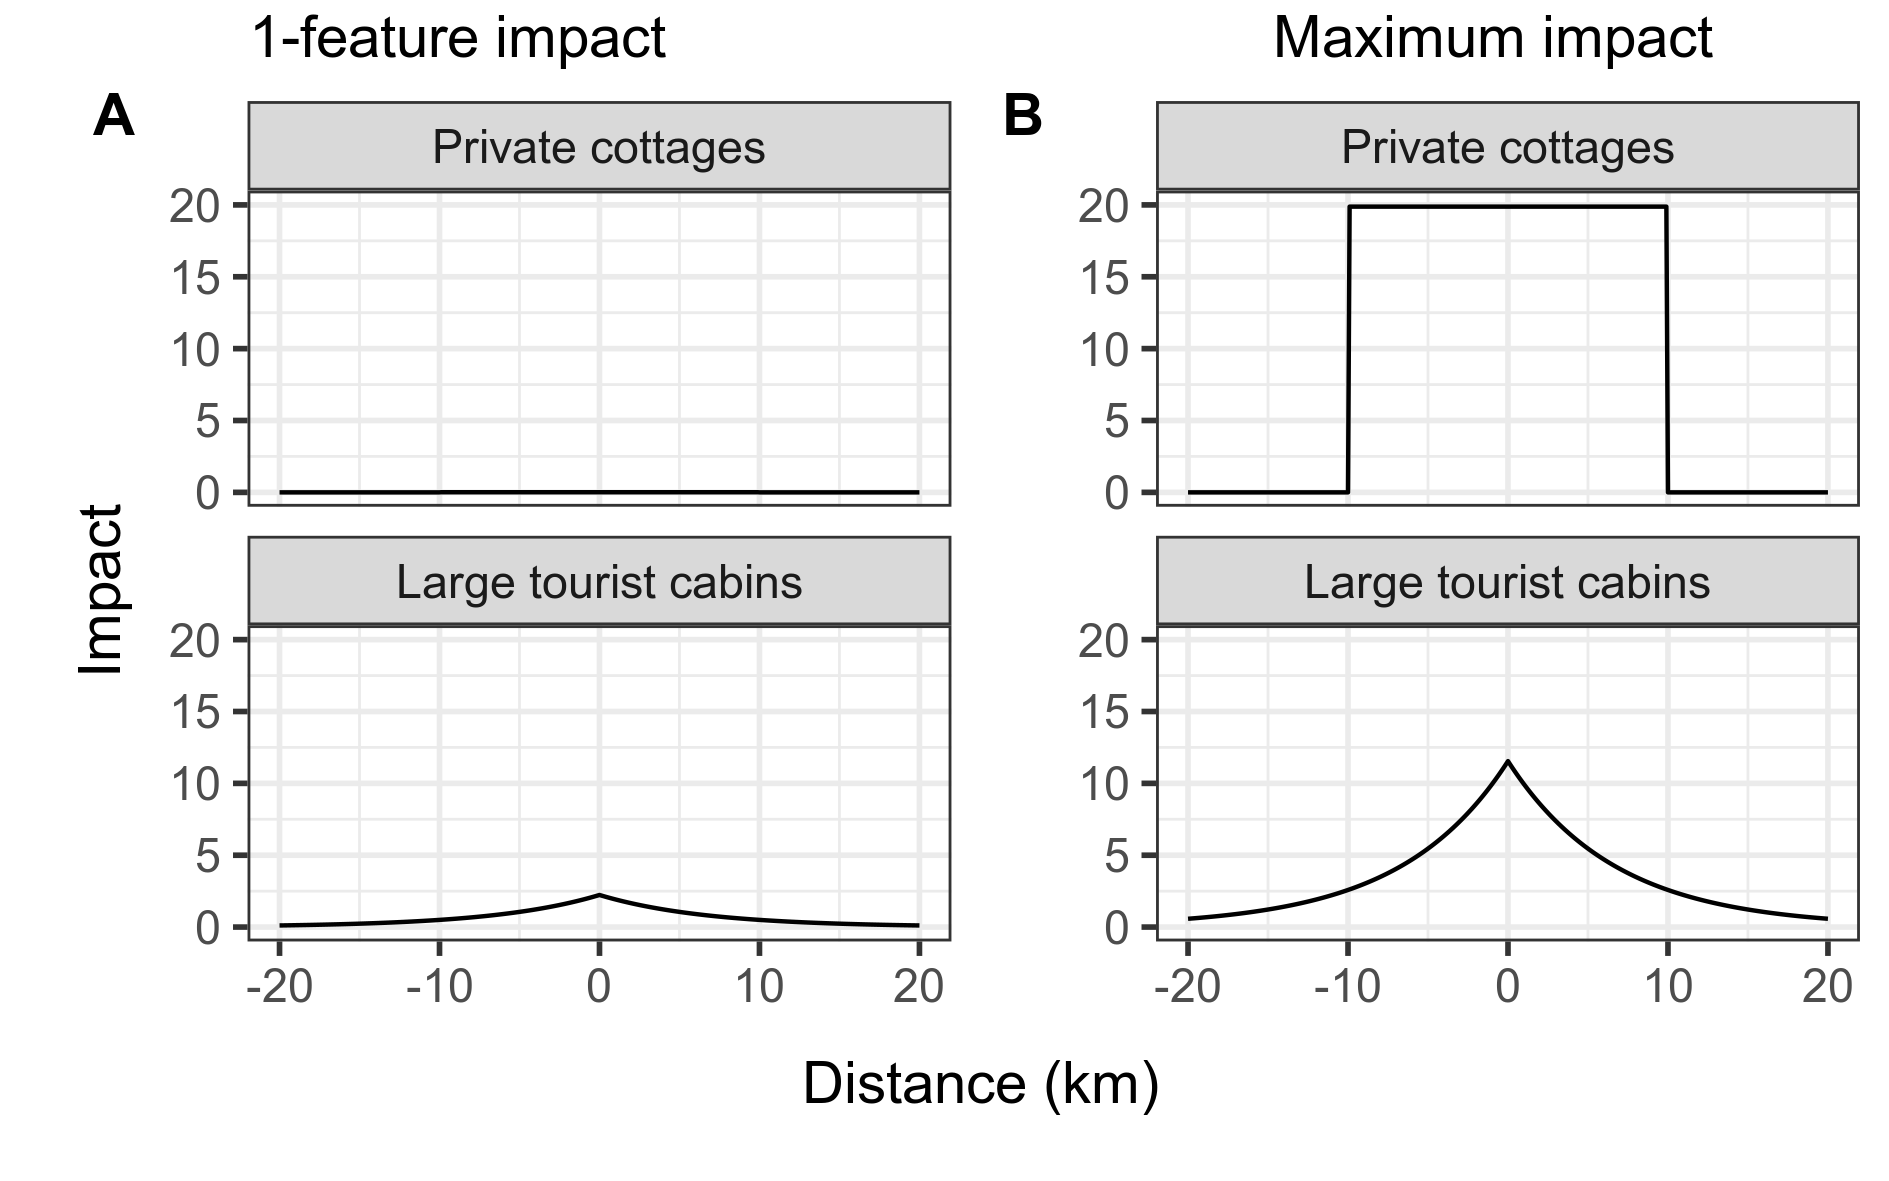
\includegraphics[width=1\textwidth,center]{figures/reindeer_zoi_impact_single_multiple_features.png}
\caption{\label{fig:impact_plot} Impact of private cottages and public cabins considering (A) only 1 feature and (B) the maximum number of features of each type of infrastructure in the study area (2664 for cottages, 5 for cabins). The impact is the product of the effect size ($\beta$) and the cumulative zone of influence ($\phi_{cumulative}$). While the impact of only one private cottage is negligible, at their maximum densities the cumulative impact of private cottages is higher than that of tourist cabins.}
\end{figure}

The estimated effect size of a single private
cottage ($\beta_{cottage} = -0.0081$) was much smaller than that of a single tourist cabin
($\beta_{\text{private cabin}} = -2.654$; Fig. \ref{fig:impact_plot}A, Table C3), as
private cottages were used by fewer people than the tourist cabins. However, as
private cottages occur at higher densities, in some areas their impact 
is larger than that of tourist cabins. In the areas where our most parsimonious model shows the 
highest cumulative ZoI of infrastructure in Hardangervidda -- where the number of private cottages sum to 2664
and the number of tourist cabins sum to 5 -- the impact of 
private cottages clusters is nearly twice that of tourist cabins
(Fig. \ref{fig:impact_plot}B and 4). Following the HSF coefficient interpretation from \citet{fieberg_how_2021}, considering that all other conditions are kept constant, a reindeer avoids an area 14.43 times more than another area with
330 fewer private cottages within a radius of 10 km. That is nearly the same difference in avoidance a reindeer presents among two areas that differ in 1 tourist cabin in a radius of 20 km (Appendix C).

When cumulative impacts of infrastructure are predicted in space by multiplying the effect size and $\phi_{cumulative}$ (eq. \ref{eqn:HSFcuminf}), we see how the relative impact of private cottages and tourist cabins changes across space. While the impact for private cottage rises to 20 in the areas with the highest cumulative ZoI of cottages, it hardly goes above 10 for tourist cabins (Fig. \ref{fig:prediction_maps}; values in the scale of predictors). Because of the combined impact of infrastructure, and given reindeer
avoided high densities of both infrastructure types at relatively large extents, 
areas of high habitat suitability for reindeer corresponded to those in which the
cumulative impact of both infrastructure is low -- which matches the
locations used by reindeer, indicated through the GPS data (Fig. \ref{fig:prediction_maps}).

\begin{figure}[h]
\centering
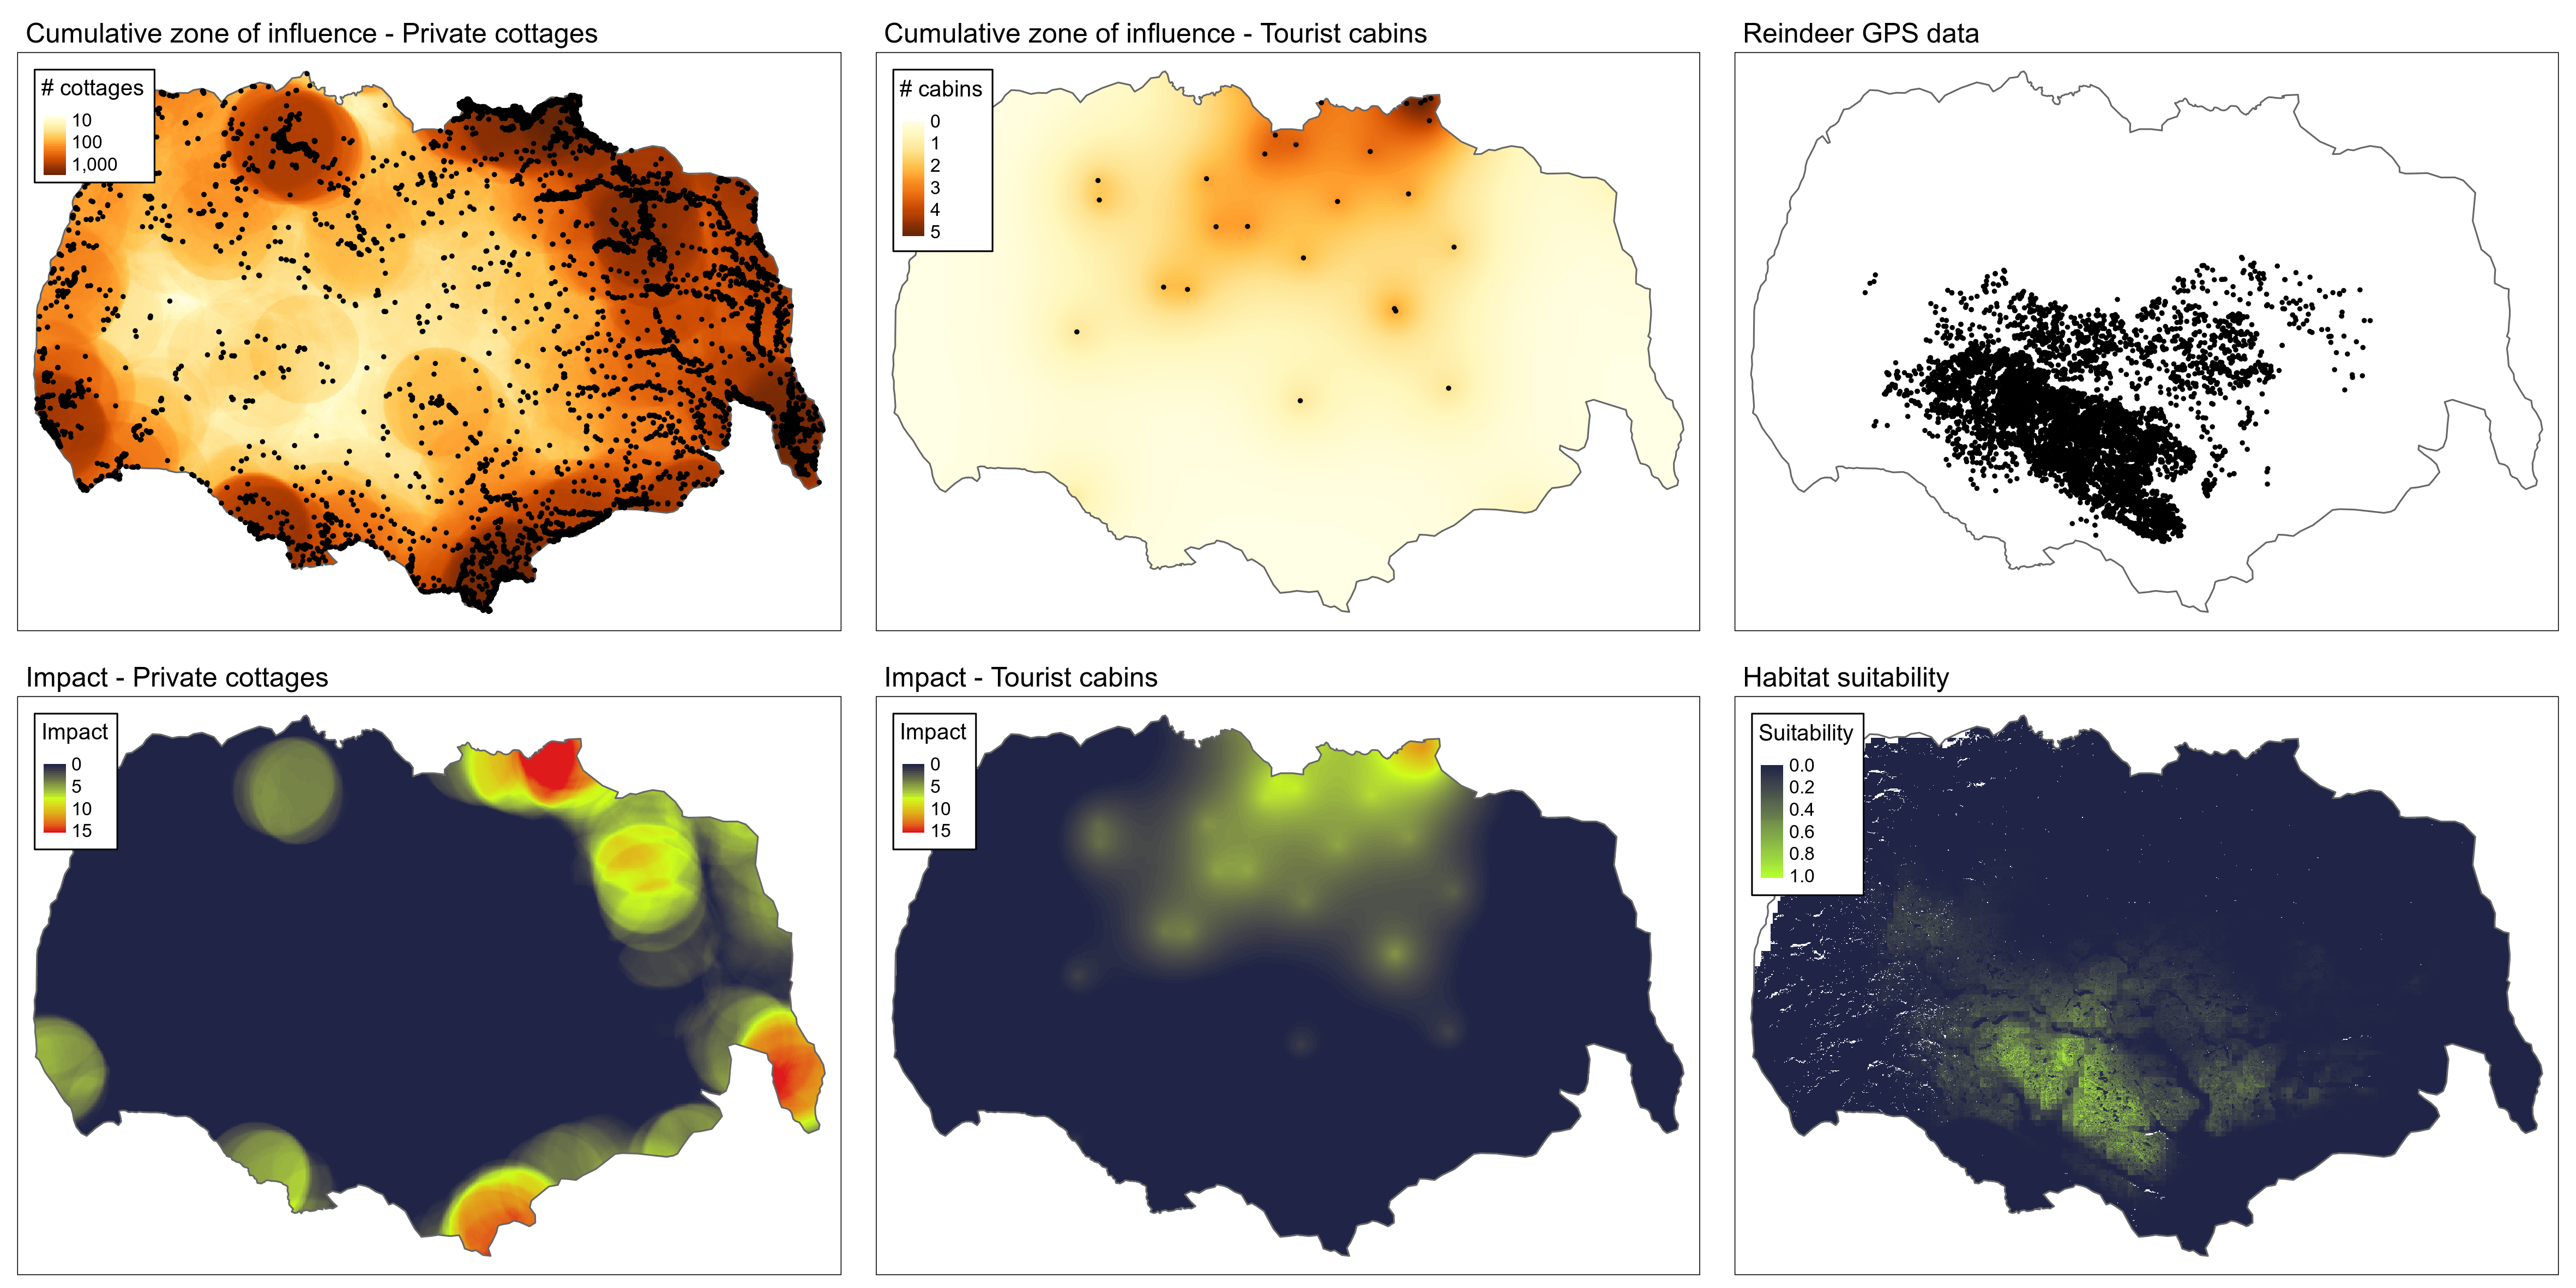
\includegraphics[width=1.3\textwidth,center]{figures/reindeer_results_prediction_maps.png}
\caption{\label{fig:prediction_maps} Maps of the most parsimonious cumulative ZoI (private cottages: threshold with 10km radius; tourist cabins: exponential decay with 20km radius) and their estimated impacts on reindeer habitat selection. These maps are showed alongside the reindeer GPS locations in the Hardengervidda wild reindeer area and the predicted reindeer habitat suitability.}
\end{figure}

\section{Discussion}

There is an urge to evaluate, debate, and inform scientists, decision-makers, and citizens about the past, current, and future impacts of global infrastructure on biodiversity \citep{laurance_conservation_2018}. Most of the decisions and regulations made for infrastructure projects are carried out with little knowledge about the potential, multiple impacts on the ecosystems where they are built and on the species living therein. Even when environmental impact assessments are well conducted, they hardly estimate the cumulative impacts of new infrastructure with existing infrastructure or new infrastructure planned in parallel \citep{laurance_roads_2017, johnson_regulating_2011}. Current approaches and tools still lack in incorporating cumulative impacts \citep[but see][for recent advances]{gillingham_integration_2016}. Thus, building upon previous frameworks \citep{naugle_unifying_2011} and adapting concepts from landscape ecology literature to measure the ZoI of the nearest and of multiple features ($\phi_{nearest}$ and $\phi_{cumulative}$), here we present a way forward to clearly assess cumulative impacts on biodiversity. 

\subsection{Applying the approach to impact assessment}

In our empirical demonstration using wild reindeer in Norway, we found strong support for the hypothesis of cumulative impacts of private cottages and tourist resorts on reindeer habitat selection, leading to large ZoI of 10 and 20 km, respectively. Quantifying impacts based on effect sizes and ZoI functions $\phi$ allows us to compare as well as to combine the effects of different types of infrastructure. Our results show that the impact of a single cottage is smaller than that of a single tourist cabin, but that the impact of several aggregated private cottages may be larger than that of tourist cabins (Fig. \ref{fig:impact_plot} and \ref{fig:prediction_maps}, Fig. C5). We also found less support for all models based only on the ZoI of the nearest feature ($\phi_{nearest}$) compared to the models incorporating the cumulative ZoI of multiple features ($\phi_{cumulative}$). This includes the models based on the log-distance to the nearest feature, which is a common proxy for the effect of spatial variables in the ecological literature \citep[e.g.][]{torres_assessing_2016,polfus_identifying_2011}. This means that, by limiting measures of infrastructure influence to the nearest feature only, researchers and practitioners have been ignoring the possibility of cumulative impacts in ecological studies and impact assessments, what limits our overall understanding of the impacts of landscape change on biodiversity.

Three points must be highlighted regarding the interpretation of the estimated ZoI.
First, if ZoI functions with different shapes are found to affect a biological response variable, the ZoI represents distinct areas affected by infrastructure. For instance, while we found a constant ZoI (threshold function) of private cabins in a radius of 10km, for tourist cabins the ZoI decays exponentially with distance, which means the radius of 20 km around the resorts are not affected homogeneously. Therefore, understanding the impact of infrastructure across space requires us to interpret the combination of effect size and ZoI (eq. \ref{eqn:HSFterm}, Fig. \ref{fig:impact_plot} and \ref{fig:prediction_maps}). Second, since the ZoI might vary according to different shapes, the area affected by infrastructure of a given type might drastically change. Indeed, in a study with bird and insect abundance, \citet{miguet_how_2017} showed that the area affected by landscape variables can increase by a factor of up to 5.7 when using a distance-weighted influence measure (as the exponential and Gaussian decay functions used here), in comparison to a threshold-based landscape measure. Third, given that the estimation of $\beta$ and $\phi$ is independent, the most likely estimated values for $\beta$ and ZoI radius can differ significantly between $\phi_{nearest}$ and $\phi_{cumulative}$, depending on the abundance and spatial distribution of features. For private cottages, which are abundant in our study area, the estimated ZoI radius for $\phi_{cumulative}$ was 10 km and the effect size was small (Fig. C3). In contrast, if only the nearest feature was considered ($\phi_{nearest}$), the estimated ZoI radius would be ten times lower (1 km) and the effect size would be several orders of magnitude higher (Fig. C3). This was not the case for tourist cabins, however, which are scarce and sparsely distributed in the study area (Fig. C4).

\subsection{Assumptions, advantages, and limitations of the approach}

As formulated here, the ZoI metrics are calculated before model fitting through the \verb|oneimpact| R package (Fig. \ref{fig:workflow}). Here lies one of the main strengths of this approach: the cumulative impact of multiple features of an infrastructure is estimated without the necessity of repeated model fitting and complex parameterization of non-linear functions \citep{lee_estimating_2020}. This allows us to estimate the ZoI for several types of infrastructure. It also allows fitting models for large datasets \citep[millions of points, e.g.][]{tucker_moving_2018} encompassing large study areas and fine resolution landscape covariates, making the approach applicable over a wide range of fields in ecology. The pre-computation of $\phi_$ makes their visualization easy and their calculation computationally efficient and flexible.

Our formulation of $\phi$ follows two main assumptions. First, the ZoI of each feature is assumed to be constant regardless of the density of points in an area. A possibly more reasonable assumption would be to consider that the ZoI of a single or few features is smaller than that of a cluster of features (e.g. for tourist cabins, clusters are expected to be used by more people and cumulatively affect a wider area). Analogous calculations with variable radius have been implemented for decades in adaptive kernel density estimation \citep{worton_kernel_1989}, so this premise can in principle be relaxed. Second, our formulation represents two extremes where only the nearest feature influences a focal ecological process ($\beta_i = 0$ for $i > 1$ in $\phi_{nearest}$) or all features affect the process equally ($\beta$ is constant over all features in $\phi_{cumulative}$). This is the simplest form of accounting for cumulative impacts of multiple features of the same type. The advantage of this formulation lies on the independence between the magnitude of the impacts ($\beta$'s) and the ZoI ($\phi$), what makes it possible to pre-compute $\phi$ before model fitting. However, more complex formulations could be extended from eq. \ref{eqn:HSFterm}, for instance by considering that the ZoI of multiple features accumulate yet the closest feature exerts a larger influence than features far away (higher $\beta$ for the nearest feature).

Through simulations, we showed that $\phi_{nearest}$ and $\phi_{cumulative}$ represent similar gradients of spatial variation when the spatial distribution of infrastructure features is sparse and the ZoI is small (the features are too spaced for their impacts to accumulate) and when the features are clustered and ZoI is large (clusters of features act as ``super-features", e.g. urban areas instead of houses; Appendix B). In these two situations, it will be difficult to assess whether the impact of multiple infrastructure features accumulate. This might be assessed prior to statistical analysis through the computation of $\phi_{nearest}$ and $\phi_{cumulative}$ with multiple ZoI and a careful evaluation of their correlations. However, as the ``true" ZoI of an infrastructure type is hardly known in advance, we recommend a general approach of computing and using both of the two ZoI metrics, to evaluate if there is evidence of cumulative impacts in the different ecological systems and processes.

The extent of the study area and the ZoIs to be evaluated must be carefully selected. First. the impact of infrastructure on ecological processes might differ depending of the extent of the study area \citep{vistnes_matter_2008}. \citet{skarin_human_2014} showed that, depending of the temporal and spatial range of the study, the same type of infrastructure might vary in their effect on biological response variables, from no effect to positive or negative effects. Second, depending on the response variable, the range of ZoI radii evaluated should extend at least the range size or the average dispersal distance of the species under study \citep{jackson_what_2012}. This is needed to ensure that the ``true" ZoI at which the ecological process being measured is affected is included among the possible ZoI, and avoid that conclusions based on an estimated ZoI that is wrong mislead management and conservation policies based on that scientific inference \citep[e.g.][]{jackson_are_2015}.

\section{Conclusions}

There is an increasing need to include cumulative impacts on environmental impact assessments and ecological studies. However, even when they are present, bringing concepts and theoretical frameworks into concrete and objective analyses to estimate cumulative impacts is often challenging and left to the responsibility of either the analysts or the regulators that review impact assessments \citep{johnson_regulating_2011}. Our approach offers resources for ecologists, environmental agencies, and stakeholders dealing with impact assessment to build concrete estimates of cumulative impacts of multiple features of an infrastructure and their zone influence. 
Even though the examples given here focused on animal space use, the cumulative impact approach we presented is applicable over a wide range
of fields within ecology. Our formulation can be easily adapted to model other types of biological responses, such as population abundance \citep[e.g.][]{benitez-lopez_impacts_2010}, species richness \citep[e.g.][]{ficetola_ecological_2009} or other measures of biological diversity and ecological processes, with direct application in environmental and strategic impact assessment and integrated land use planning.
      
\section*{Acknowledgements}

We thank C. Johnson for discussions on cumulative impact concepts, P. Dodonov, M.H. Vancine, and J. Nowosad for discussion around the implementation ZoI metrics in R, R. Muylaert and M. Grainger for a critical review of the text, and E. Gurarie for the incentive and teachings on how to build an R package. We are grateful to several local projects allowing to collect reindeer GPS data in Norway in the past decades. The work presented here is the
result of large research projects supported by the Research Council of Norway: OneImpact (n. 287925), RenewableReindeer (n. 243746), and ProdChange (n. 255635). BBN, AS, PS, and MA were also supported by a grant from the Swedish Energy Agency within the research programme Vindval (grant n. 46780-1) and by project MineDeer (Vinnova project n. 2019-05191).

\section*{Conflicts of Interest}

The authors declare no conflicts of interest.

\section*{Authors’ contributions}

BBN, BVM, and MP conceived the idea and designed the methods, with contributions from TT, ASt, MA, and ASk; BBN, BVM, MP, TT, KL, and OS collected and provided the data; BBN, BVM, and MP analyzed the data and interpreted the results; BBN and BVM led the writing of the manuscript. All authors contributed critically in discussions and to the drafts, and gave final approval for publication.

\section*{Data availability statement}

GPS data is archived in Movebank (www.movebank.org) and can be accessed upon request. All environmental data was retrieved from public repositories. The \verb|oneimpact| package is open and available at \url{github.com/NINAnor/oneimpact}, and all scripts used in the analyses are available in the Github repository \url{github.com/bniebuhr/cumulative_zoi_paper}.

\section*{Supplementary Material}

Appendix A. Defining and deriving the zone of influence for multiple infrastructure features \\
Appendix B. Comparing the zone of influence of the nearest feature with the cumulative zone of influence of multiple features \\
Appendix C. Cumulative impacts of infrastructure on reindeer space use: fitting habitat selection models \\
Appendix D. Getting started with the \verb|oneimpact| package \\

\bibliographystyle{besjournals}
\bibliography{cumzoi_bib}

\end{document}
